\documentclass{beamer}

\mode<presentation> {
\usetheme{Warsaw}
\usecolortheme{seahorse}
}

\usepackage{subcaption}
\usepackage{tcolorbox}
\tcbuselibrary{skins}
\usepackage[table]{xcolor}
\usepackage{colortbl}
\usepackage{array, multirow, multicol, tabularx}
\usepackage{booktabs}
\usepackage{amsfonts}
\usepackage{amsmath}
\usepackage{amssymb}
\usepackage{setspace}
\usepackage{caption}
\usepackage{ragged2e}
\usepackage{bm}
\usefonttheme[onlymath]{serif}
\usepackage{amsthm}
\usepackage{textcomp}
\usepackage{graphicx}
\usepackage{tikz}
\usepackage{pifont}
\usetikzlibrary{shapes, positioning, calc, arrows.meta}
\usepackage{pgfplots}
\pgfplotsset{compat=1.18}
\usepackage[outline]{contour}
\setbeamertemplate{caption}[numbered]

% Colors (same values as the paper)
\definecolor{morado}{rgb}{.88,.50,.90}
\definecolor{darkgreen}{rgb}{0,0.39,0}
\definecolor{matlabBlue}{rgb}{0.000,0.380,0.900}

% Modern palette for the motivation schematic
\definecolor{primaryblue}{RGB}{37, 99, 235}
\definecolor{darkslate}{RGB}{15, 23, 42}
\definecolor{crimsonred}{RGB}{220, 38, 38}
\definecolor{forestgreen}{RGB}{22, 163, 74}
\definecolor{lightgraybg}{RGB}{248, 250, 252}
\definecolor{amberbg}{RGB}{217, 119, 6}

% Swatches for figure legends (same as the paper)
\DeclareRobustCommand{\legsolid}[1]{\textcolor{#1}{\rule[0.55ex]{1.6em}{0.8pt}}}
\DeclareRobustCommand{\legdotted}[1]{\textcolor{#1}{\makebox[1.6em][l]{\dotfill}}}

% Reference line at the bottom of a slide
\newcommand{\slideref}[1]{\vfill{\tiny #1}}

% Make the Warsaw head/foot slimmer (keep them visible, but reduce height)
\setbeamertemplate{headline}{%
  \leavevmode%
  \hbox{%
    \begin{beamercolorbox}[wd=\paperwidth,ht=2.1ex,dp=0.9ex]{section in head/foot}%
      \scriptsize\insertnavigation{\paperwidth}%
    \end{beamercolorbox}%
  }%
}

\setbeamertemplate{footline}{%
  \leavevmode%
  \hbox{%
    \begin{beamercolorbox}[wd=.72\paperwidth,ht=2.1ex,dp=0.9ex,left]{author in head/foot}%
      \scriptsize\hspace*{1ex}\insertshortauthor
    \end{beamercolorbox}%
    \begin{beamercolorbox}[wd=.18\paperwidth,ht=2.1ex,dp=0.9ex,center]{title in head/foot}%
      \scriptsize\insertshorttitle
    \end{beamercolorbox}%
    \begin{beamercolorbox}[wd=.10\paperwidth,ht=2.1ex,dp=0.9ex,right]{date in head/foot}%
      \scriptsize\insertframenumber/\inserttotalframenumber\hspace*{1ex}
    \end{beamercolorbox}%
  }%
  \vskip0pt%
}

\title[{October 26-28, 2026 CDMX, México}]{Neuromorphic Modeling and Control for a Coaxial Hexarotor UAV using Spiking Neural Networks}
\author[{XXVIII Congreso Mexicano de Robótica}]
{
    \texorpdfstring{
    \\ \textbf{Anel Olivares}, Gandhi Torres, Victor J. Silva\\ Eduardo S. Espinoza, Juan M. Bustamante, and Patricio Ordaz \\
    \vspace{0.15cm}
    \begin{center}
        \includegraphics[scale = .2]{images_comrob/Comrob_logo.png}
    \end{center}
   }
   { }
}
\date[October 2026]{}

\begin{document}
\contourlength{0.01cm}

\begin{frame}
    \titlepage
\end{frame}

\begin{frame}
    \frametitle{Content}
    % Show subsections so the Problem statement appears in the outline
    \tableofcontents
\end{frame}

%===================================================================
\section{Introduction}

\subsection{Problem statement}

%------------------------------------------------
% ============================================================
% Motivation — Von Neumann vs. Neuromorphic Computing
% ============================================================
\begin{frame}{Why Neuromorphic Computing?}

% Subtitle
\begin{center}
{\small\color{gray!80!black}\textbf{Rethinking how intelligent machines compute}}
\end{center}

\vspace{-0.2cm}

\centering
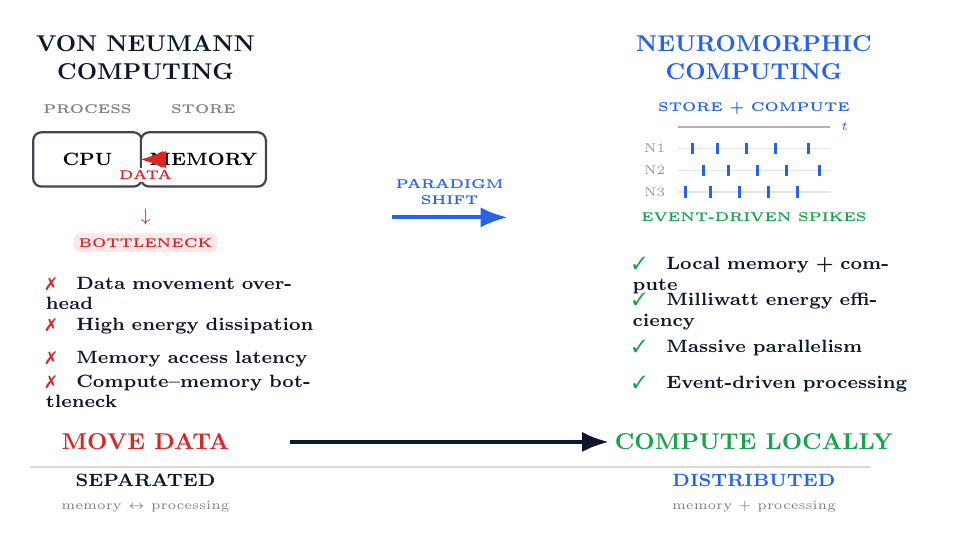
\begin{tikzpicture}[
    font=\scriptsize,
    scale=0.92,
    transform shape,
    >=Latex,
    cpubox/.style={
        draw=darkslate!80,
        fill=white,
        rounded corners=3pt,
        minimum width=1.5cm,
        minimum height=0.75cm,
        line width=0.8pt,
        font=\bfseries\scriptsize
    },
    cardbox/.style={
        draw=gray!30,
        fill=lightgraybg,
        rounded corners=6pt,
        line width=0.8pt
    }
]

% ============================================================
% HEADERS
% ============================================================
\node[font=\bfseries\small, align=center, text=darkslate] at (-4.2, 2.8) {VON NEUMANN\\COMPUTING};
\node[font=\bfseries\small, align=center, text=primaryblue] at (4.2, 2.8) {NEUROMORPHIC\\COMPUTING};

% ============================================================
% LEFT — VON NEUMANN
% ============================================================
\node[font=\tiny\bfseries, text=gray] at (-5.0, 2.1) {PROCESS};
\node[font=\tiny\bfseries, text=gray] at (-3.4, 2.1) {STORE};

\node[cpubox] (cpu) at (-5.0, 1.4) {CPU};
\node[cpubox] (memory) at (-3.4, 1.4) {MEMORY};

% Heavy data movement arrow
\draw[<->, line width=1.2pt, color=crimsonred] (cpu.east) -- (memory.west);
\node[font=\tiny\bfseries, text=crimsonred, fill=white, inner sep=1pt] at (-4.2, 1.18) {DATA};

% Bottleneck callout
\node[font=\scriptsize\bfseries, text=crimsonred] at (-4.2, 0.6) {$\downarrow$};
\node[font=\tiny\bfseries, fill=crimsonred!10, text=crimsonred, rounded corners=2pt, inner sep=2pt] at (-4.2, 0.25) {BOTTLENECK};

% Problems list
\node[anchor=west, text width=3.8cm] at (-5.7,-0.45) {\color{crimsonred}\ding{55}\quad \textbf{\color{darkslate}Data movement overhead}};
\node[anchor=west, text width=3.8cm] at (-5.7,-0.90) {\color{crimsonred}\ding{55}\quad \textbf{\color{darkslate}High energy dissipation}};
\node[anchor=west, text width=3.8cm] at (-5.7,-1.35) {\color{crimsonred}\ding{55}\quad \textbf{\color{darkslate}Memory access latency}};
\node[anchor=west, text width=3.8cm] at (-5.7,-1.80) {\color{crimsonred}\ding{55}\quad \textbf{\color{darkslate}Compute--memory bottleneck}};

% ============================================================
% CENTER — PARADIGM SHIFT
% ============================================================
\draw[->, line width=1.5pt, color=primaryblue] (-0.8, 0.6) -- (0.8, 0.6);
\node[font=\tiny\bfseries, text=primaryblue, align=center] at (0, 0.95) {PARADIGM\\SHIFT};

% ============================================================
% RIGHT — NEUROMORPHIC COMPUTING
% ============================================================
\node[font=\tiny\bfseries, text=primaryblue] at (4.2, 2.1) {STORE + COMPUTE};

% Spiking raster plot
\draw[gray!60, line width=0.6pt] (3.15, 1.85) -- (5.25, 1.85);
\node[font=\tiny, text=primaryblue, anchor=west] at (5.28, 1.85) {$t$};

\foreach \y/\lab in {1.55/N1, 1.25/N2, 0.95/N3}{
    \node[font=\tiny, text=gray!80, anchor=east] at (3.10,\y) {\lab};
    \draw[gray!20, line width=0.4pt] (3.15,\y) -- (5.25,\y);
}

% Spike ticks
\foreach \x in {3.35, 3.70, 4.10, 4.50, 4.95}{
    \draw[line width=1.0pt, color=primaryblue] (\x,1.55-0.08) -- (\x,1.55+0.08);
}
\foreach \x in {3.50, 3.85, 4.25, 4.65, 5.10}{
    \draw[line width=1.0pt, color=primaryblue] (\x,1.25-0.08) -- (\x,1.25+0.08);
}
\foreach \x in {3.25, 3.60, 4.00, 4.40, 4.80}{
    \draw[line width=1.0pt, color=primaryblue] (\x,0.95-0.08) -- (\x,0.95+0.08);
}

\node[font=\tiny\bfseries, text=forestgreen] at (4.2, 0.6) {EVENT-DRIVEN SPIKES};

% Advantages list
\node[anchor=west, text width=4.0cm] at (2.4,-0.20) {\color{forestgreen}\ding{51}\quad \textbf{\color{darkslate}Local memory + compute}};
\node[anchor=west, text width=4.0cm] at (2.4,-0.70) {\color{forestgreen}\ding{51}\quad \textbf{\color{darkslate}Milliwatt energy efficiency}};
\node[anchor=west, text width=4.0cm] at (2.4,-1.20) {\color{forestgreen}\ding{51}\quad \textbf{\color{darkslate}Massive parallelism}};
\node[anchor=west, text width=4.0cm] at (2.4,-1.70) {\color{forestgreen}\ding{51}\quad \textbf{\color{darkslate}Event-driven processing}};

% ============================================================
% MAIN TAKEAWAY BANNER
% ============================================================
\node[font=\small\bfseries, text=crimsonred] at (-4.2, -2.5) {MOVE DATA};
\draw[->, line width=1.5pt, color=darkslate] (-2.2, -2.5) -- (2.2, -2.5);
\node[font=\small\bfseries, text=forestgreen] at (4.2, -2.5) {COMPUTE LOCALLY};

% ============================================================
% BOTTOM ARCHITECTURAL CONTRAST
% ============================================================
\draw[gray!30, line width=0.6pt] (-5.8, -2.85) -- (5.8, -2.85);

\node[align=center, font=\scriptsize] at (-4.2, -3.2) {
    \textbf{\color{darkslate}SEPARATED}\\[1pt]
    {\tiny\color{gray}memory $\leftrightarrow$ processing}
};

\node[align=center, font=\scriptsize] at (4.2, -3.2) {
    \textbf{\color{primaryblue}DISTRIBUTED}\\[1pt]
    {\tiny\color{gray}memory + processing}
};

\end{tikzpicture}

\end{frame}

%------------------------------------------------
\begin{frame}{State of the art and gap}
\footnotesize
\begin{itemize}
    \item NEF-based SNN controllers have been used on underactuated systems and quadrotor UAVs\textsuperscript{1,2}.
    \item Neuromorphic control on Intel Loihi for a robotic arm\textsuperscript{3}.
    \item SNN flight control on neuromorphic hardware is limited to reduced-order cases: 1-DOF attitude\textsuperscript{4} and single-axis vertical landing\textsuperscript{5}.
\end{itemize}

\begin{table}[h]
    \centering
    \begin{tcolorbox}[
        tabularx = {l | X},
        title = Gap:,
        colback = primaryblue!8,
        colframe = primaryblue,
        fontupper=\footnotesize
    ]
        $\star$ & In these works the vehicle dynamics are simulated \textbf{outside} the neural framework.\\
        $\star$ & A fully neuromorphic architecture (dynamics \textbf{and} cascade controller in the NEF) has received little attention, especially beyond the quadrotor.\\
    \end{tcolorbox}
\end{table}

\slideref{[1] O. A. Garcia \emph{et al.}, CCE 2023. \quad [2] A. Olivares \emph{et al.}, IFAC-PapersOnLine, 2025; Neural Comput.\ Appl., 2026. \quad [3] T. DeWolf \emph{et al.}, Neuromorph.\ Comput.\ Eng., 2023. \quad [4] R. K. Stagsted \emph{et al.}, IROS 2020. \quad [5] J. Dupeyroux \emph{et al.}, ICRA 2021.}
\end{frame}

%------------------------------------------------

%------------------------------------------------
\begin{frame}{Problem and Contributions}

\centering
\vspace{-0.45cm}

{\scriptsize\bfseries\color{primaryblue}RESEARCH QUESTION\par}
\vspace{0.08cm}

{\normalsize\color{darkslate}
\parbox{0.96\linewidth}{\centering
Can the \textbf{\color{primaryblue}full flight stack} of a \textbf{coaxial hexarotor}
be realized inside a \textbf{\color{primaryblue}spiking SNN} without degrading
closed-loop tracking?}\par}

\vspace{0.18cm}

{\scriptsize\bfseries\color{primaryblue}CONTRIBUTIONS\par}
\vspace{0.06cm}

{\small
\begin{itemize}\setlength\itemsep{4pt}
    \item[\textcolor{primaryblue}{\ding{51}}] \textbf{Full stack in NEF/Nengo}: model + cascade control realized as a spiking network.
    \item[\textcolor{primaryblue}{\ding{51}}] \textbf{Validation}: trajectory tracking vs. MATLAB/Simulink baseline.
    \item[\textcolor{primaryblue}{\ding{51}}] \textbf{Modularity}: decoupled control modules across UAV subsystems.
\end{itemize}
}

\end{frame}

%------------------------------------------------
% Visual separator slide (T6 coaxial figure only)
\begin{frame}{T6 coaxial hexarotor}
\centering
\includegraphics[width=\linewidth,height=0.78\textheight,keepaspectratio]{images_hexa/dinamica_hexa3.pdf}
\end{frame}

%------------------------------------------------
\begin{frame}{Cascade control scheme}
\centering
\vspace{-0.55cm}
\hspace*{-0.02\linewidth}%
\includegraphics[width=1.04\linewidth,height=0.90\textheight,keepaspectratio]{images_hexa/cascade_classic.pdf}
\end{frame}






%===================================================================
\section{Dynamic modeling of the coaxial hexarotor}

\subsection{Newton--Euler formulation}
\begin{frame}{Newton--Euler formulation}
\begin{columns}
\column{6.2cm}
\small
Rigid-body dynamics:
\begin{align*}
\dot{\bm{\xi}} &= \bm{V}, & m\dot{\bm{V}} &= \bm{R}\bm{F},\\
\dot{\bm{R}} &= \bm{R}\hat{\bm{\Omega}}, & \mathbb{I}\dot{\bm{\Omega}} &= -\bm{\Omega}\times\mathbb{I}\bm{\Omega}+\bm{\Gamma}
\end{align*}
Virtual inputs (T6, coaxial pairs $(f_1,f_2)$, $(f_3,f_4)$, $(f_5,f_6)$):
\begin{align*}
u &= \textstyle\sum_{i=1}^{6} f_i\\
\Gamma_\phi &= l_1(f_1+f_2-f_5-f_6)\\
\Gamma_\theta &= l_2(f_1+f_2+f_5+f_6)-l_3(f_3+f_4)\\
\Gamma_\psi &= (\gamma_1+\gamma_3+\gamma_5)-(\gamma_2+\gamma_4+\gamma_6)
\end{align*}

\column{4.8cm}
\begin{tcolorbox}[colback=morado!10,colframe=morado!80,left=0.8mm,right=0.8mm,top=0.6mm,bottom=0.6mm]
\scriptsize
\textbf{Mental map:}
\begin{itemize}\setlength\itemsep{0pt}
    \item $(f_i,\gamma_i)\ \rightarrow\ (u,\bm{\Gamma})\ \rightarrow\ (\bm{\Omega},\bm{R})$
    \item $\bm{R}\bm{F}\ \rightarrow\ \dot{\bm{V}}\ \rightarrow\ \bm{\xi}$
\end{itemize}
\textbf{Where:} $\bm{\xi}$ position, $\bm{\eta}$ Euler angles, $\bm{\Omega}$ body rates, $\bm{R}$ rotation, $l_{1,2,3}$ moment arms.
\\[0.05cm]
\textbf{Assumptions:} near-hover; aerodynamics/wind/actuator dynamics neglected.
\end{tcolorbox}
\end{columns}
\end{frame}

\subsection{Reduced subsystems}
\begin{frame}{Decomposition into four subsystems}
With the altitude control law and $\psi\approx 0$ (small angles), the dynamics reduce to:
\begin{table}[h]
    \centering
    \renewcommand{\arraystretch}{1.5}
    \begin{tabular}{lll}
        \hline
        \textbf{Subsystem} & \textbf{Translational} & \textbf{Rotational}\\ \hline \hline
        Altitude & $\ddot z = -\dfrac{u}{m}\cos\theta\cos\phi + g$ & -- \\
        Longitudinal & $\ddot x = -g\tan\theta$ & $\ddot\theta = \Gamma_\theta/I_{yy}$\\
        Lateral & $\ddot y = g\tan\phi/\cos\theta$ & $\ddot\phi = \Gamma_\phi/I_{xx}$\\
        Directional & -- & $\ddot\psi = \Gamma_\psi/I_{zz}$\\
        \hline \hline
    \end{tabular}
\end{table}
\end{frame}
\subsection{Neural representation in Nengo}


\begin{frame}{Nonlinear dynamics as a recurrent population}
\begin{columns}
\column{4.6cm}
\begin{block}{Recurrent spiking population}
    \centering
    \includegraphics[width=\linewidth]{images_hexa/NLS_population.pdf}
\end{block}
\scriptsize
$h(t)=\frac{1}{\tau}e^{-t/\tau}$: synaptic filter,\\ $\tau$: synaptic time constant.
\column{6.3cm}
\small
With $W(t)=F'(\chi)+G'(\upsilon)$ and $\chi = h * W$:
\begin{equation*}
\dot \chi = \frac{1}{\tau}\bigl[F'(\chi)- \chi + G'(\upsilon)\bigr]
\end{equation*}
Matching it with $\dot\chi = F(\chi)+G(\upsilon)$ gives
\begin{tcolorbox}[colback = morado!10, colframe = morado!80, left=1mm, right=1mm]
\begin{equation*}
F'(\chi)= \tau F(\chi) + \chi, \quad G'(\upsilon) = \tau G(\upsilon)
\end{equation*}
\end{tcolorbox}
\end{columns}
\end{frame}

\begin{frame}{One neural template for the six subsystems}
For $\chi=[\zeta,\dot\zeta]^\top$, $\zeta\in\{z,x,\theta,y,\phi,\psi\}$:
\begin{equation*}
F'_\zeta(\chi)=
\begin{bmatrix} \chi_1+\tau\chi_2\\ \chi_2 \end{bmatrix},
\qquad
G'_\zeta(\upsilon_\zeta)=\tau
\begin{bmatrix} 0\\ \upsilon_\zeta \end{bmatrix}
\end{equation*}
Only the input function $\upsilon_\zeta$ changes:
\begin{table}[h]
    \centering
    \begin{tcolorbox}[
        tabularx = {l | l || l | l},
        colback = morado!10,
        colframe = morado!80
    ]
        $\zeta$ & $\upsilon_\zeta$ & $\zeta$ & $\upsilon_\zeta$\\
        \hline \hline
        $z$ & $-u\cos\theta\cos\phi/m+g$ & $\theta$ & $\Gamma_\theta/I_{yy}$\\
        $x$ & $-g\tan\theta$ & $\phi$ & $\Gamma_\phi/I_{xx}$\\
        $y$ & $g\tan\phi/\cos\theta$ & $\psi$ & $\Gamma_\psi/I_{zz}$\\
    \end{tcolorbox}
\end{table}
$\Rightarrow$ a modular and scalable neuromorphic model of the hexarotor.
\end{frame}

%===================================================================
\section{Control architecture}

\subsection{Classic cascade controller}
\begin{frame}{Cascade control scheme}
\centering
% No block/background: keeps the figure on pure white
\includegraphics[width=\linewidth,height=0.82\textheight,keepaspectratio]{images_hexa/cascade_classic.pdf}
\end{frame}

\begin{frame}{Classic control laws}
\small
\textbf{Altitude} (feedback linearization, PID):
\begin{equation*}
u= \frac{m}{\cos\theta \cos \phi}\Bigl( g - \underbrace{\bigl(k_{p_z} e_z+k_{d_z} \dot e_z +k_{i_z}\textstyle\int e_z\,dt\bigr)}_{u_z}\Bigr)
\end{equation*}
\textbf{Outer loops} (PID) $\rightarrow$ desired angles:
\begin{equation*}
\theta_d=-\tan^{-1}\!\left(\frac{u_x}{g}\right),\qquad
\phi_d=\tan^{-1}\!\left(\frac{u_y\cos\theta}{g}\right)
\end{equation*}
\textbf{Inner loops} (PD):
\begin{equation*}
\Gamma_\theta = I_{yy}\underbrace{(k_{p_\theta}e_\theta+k_{d_\theta}\dot e_\theta)}_{u_\theta},\quad
\Gamma_\phi = I_{xx}\underbrace{(k_{p_\phi}e_\phi+k_{d_\phi}\dot e_\phi)}_{u_\phi},
\end{equation*}
\vspace{-0.3cm}
\begin{equation*}
\Gamma_\psi = I_{zz}\underbrace{(k_{p_\psi}e_\psi+k_{d_\psi}\dot e_\psi)}_{u_\psi}
\end{equation*}
with $e_\zeta=\zeta_d-\zeta$ and $\dot e_\zeta=\dot\zeta_d-\dot\zeta$.
\end{frame}

\subsection{Neural controller}
\begin{frame}{Neural controller: error and derivative term}
\begin{itemize}
    \item Translational loops $u_x,u_y,u_z$: \textbf{neural PID} (remove steady-state error).
    \item Attitude loops $u_\phi,u_\theta,u_\psi$: \textbf{neural PD} (no integral action needed).
\end{itemize}
The error $e_\zeta$ is computed with an excitatory connection (reference $\zeta_d$) and an inhibitory connection (measured $\zeta$). The derivative uses the Euler approximation\textsuperscript{1}:
\begin{equation*}
\dot e_\zeta \approx \textcolor{darkgreen}{\Delta e_\zeta} = \frac{e_\zeta(\tau)-e_\zeta(2\tau)}{\tau}
\end{equation*}
One connection provides the excitatory feedforward signal $e_\zeta(\tau)$; the inhibitory one, $e_\zeta(2\tau)$, has a longer time constant.
\slideref{[1] A. Olivares \emph{et al.}, ``Biologically-inspired self-tuning neuromorphic PID control for real-time trajectory tracking of a UAS,'' IFAC-PapersOnLine, 2025.}
\end{frame}

\begin{frame}{Neural controller: integral term}
The integral action of the translational loops is a neural integrator\textsuperscript{1}:
\begin{align*}
    \dot{\mathbf{x}}_\xi &= \mathbf{A}\mathbf{x}_\xi + \mathbf{B}\nu_\xi
\end{align*}
\begin{tcolorbox}[
    tabularx = {l},
    colback = morado!10,
    colframe = morado!80
]
    NEF mapping:\\
    \hline \hline
    $\mathbf{A}_{\text{neu}} = \tau \mathbf{A} + \mathbf{I}, \quad \mathbf{B}_{\text{neu}} = \tau \mathbf{B}$\\
    Pure integrator: $\mathbf{A} = \mathbf{0}$, $\mathbf{B} = \mathbf{I}$\\
    $\Rightarrow \mathbf{A}_{\text{neu}} = \mathbf{I}, \quad \mathbf{B}_{\text{neu}} = \tau \mathbf{K}_i$\\
\end{tcolorbox}
The gain $\mathbf{K}_i$ is applied to the input \textbf{before} the neural integration stage.
\slideref{[1] A. Olivares \emph{et al.}, ``Self-tuning neuromorphic controller for real-time UAS trajectory tracking based on prescribed error sensitivity,'' Neural Comput.\ Appl., 2026.}
\end{frame}

\begin{frame}{Complete neuromorphic flight-control architecture}
\centering
% No block/background: keeps the figure on pure white
\includegraphics[width=\linewidth,height=0.82\textheight,keepaspectratio]{images_hexa/Digrama_UAV_dinamyc_ZXTheta-YPhi-3.pdf}

\vspace{0.05cm}
\tiny Nonlinear couplings are computed in shared ensembles, e.g.\ $\phi_d=\tan^{-1}(u_y\cos\theta/g)$ and $\upsilon_y = g\tan\phi/\cos\theta$.
\end{frame}

%===================================================================
\section{Simulation results}

% Mission description and gain tables removed to keep the results section figure-focused.


\subsection{Tracking results}
\begin{frame}{Closed-loop states}
\begin{columns}[T,onlytextwidth]
\column{0.78\textwidth}
\centering
\includegraphics[width=\linewidth,height=0.78\textheight,keepaspectratio]{images_hexa/fig01_states_v5_rad.pdf}

\column{0.22\textwidth}
\footnotesize
\legdotted{black} Ref.\\
\legsolid{matlabBlue} Classic\\
\legsolid{red} SNN/Nengo
\end{columns}
\end{frame}

\begin{frame}{Control commands}
\begin{columns}[T,onlytextwidth]
\column{0.78\textwidth}
\centering
\includegraphics[width=\linewidth,height=0.78\textheight,keepaspectratio]{images_hexa/fig02_commands_v5_rads2.pdf}

\column{0.22\textwidth}
\footnotesize
\legsolid{matlabBlue} Classic\\
\legsolid{red} SNN/Nengo
\end{columns}
\end{frame}

\subsection{Performance indices}
\begin{frame}{Tracking performance over the 60\,s mission}
\begin{table}[h!]
\centering
\small
\begin{tabular}{lcccc}
\toprule
 & \multicolumn{2}{c}{RMSE} & \multicolumn{2}{c}{ISE} \\
\cmidrule(lr){2-3}\cmidrule(lr){4-5}
Variable & Classic & SNN & Classic & SNN \\
\midrule
$x$ [m]        & $0.008$ & $0.032$ & $3.95 \times 10^{-3}$ & $0.0627$ \\
$y$ [m]        & $0.013$ & $0.033$ & $0.0101$ & $0.0660$ \\
$z$ [m]        & $0.019$ & $0.048$ & $0.0213$ & $0.1367$ \\
$\theta$ [rad] & $3.26 \times 10^{-4}$ & $0.005$ & $6.38 \times 10^{-6}$ & $1.71 \times 10^{-3}$ \\
$\phi$ [rad]   & $9.73 \times 10^{-4}$ & $0.012$ & $5.68 \times 10^{-5}$ & $8.67 \times 10^{-3}$ \\
$\psi$ [rad]   & $6.62 \times 10^{-3}$ & $0.009$ & $2.63 \times 10^{-3}$ & $4.61 \times 10^{-3}$ \\
\bottomrule
\end{tabular}
\end{table}
\begin{tcolorbox}[colback = morado!10, colframe = morado!80, title = SNN vs.\ classic correlation $\rho_{\mathrm{SNN,cls}}$]
\centering
$x$: 0.9993 \qquad $y$: 0.9998 \qquad $-z$: 0.9992
\end{tcolorbox}
\end{frame}

\begin{frame}{Discussion}
\begin{itemize}
    \item $\rho_{\mathrm{SNN,cls}} > 0.999$: the SNN reproduces the dynamics of the classic controller.
    \vspace{0.2cm}
    \item Position RMSE stays below 5\,cm, but the SNN has higher RMSE and ISE than the classic baseline on every variable.
    \vspace{0.2cm}
    \item These differences are consistent with known limitations of the NEF\textsuperscript{1}:
    \begin{itemize}
        \item decoding errors from finite neural ensembles;
        \item LIF vs.\ rectified-linear activation functions;
        \item bounded maximum firing rates $\rightarrow$ saturation for large inputs.
    \end{itemize}
\end{itemize}
\vspace{0.3cm}
\small Source code and gains: \texttt{github.com/esteedeq/UAV\_Nengo}
\slideref{[1] T. DeWolf \emph{et al.}, ``Neuromorphic control of a simulated 7-DOF arm using Loihi,'' Neuromorph.\ Comput.\ Eng., 2023.}
\end{frame}

%===================================================================
\section{Conclusions}

\begin{frame}{Conclusions and future work}
\begin{itemize}
    \item A neuromorphic modeling and control framework for a coaxial hexarotor UAV was presented: the reduced nonlinear dynamics \textbf{and} the cascade flight controller are implemented as SNNs with the NEF and Nengo.
    \vspace{0.2cm}
    \item In a 60\,s trajectory-tracking simulation, the SNN controller closely reproduced the conventional MATLAB/Simulink implementation ($\rho > 0.99$ in the translational axes).
    \vspace{0.2cm}
    \item \textbf{Limitations:} simulation only; reduced model without rotor-level aerodynamics, actuator dynamics or external disturbances.
    \vspace{0.2cm}
    \item \textbf{Future work:} complete UAV dynamics, disturbances and uncertainties, and implementation on neuromorphic hardware for real-time experiments.
\end{itemize}
\end{frame}

\begin{frame}
    \begin{center}
    \textbf{\Huge Thank you for your attention}
    \end{center}
\end{frame}

\end{document}
